\documentclass[letterpaper]{article}
\usepackage{natbib,alife13}

\title{Aracna: An Open-Source Quadruped Platform for Evolutionary Robotics}
\author{Sara Lohmann, Eric Gold, Jason Yosinski, Jeremy Blum \and Hod Lipson \\
\mbox{}\\
Cornell University, 239 Upson Hall, Ithaca, NY 14853 \\
\texttt{sml253@cornell.edu}}



\begin{document}
\maketitle

\begin{abstract}
We describe a new, quadruped robot platform, Aracna,
which requires non-intuitive motor commands in order to locomote and thus provides an interesting challenge for gait learning algorithms, such as those frequently developed in the Evolutionary Computation and Artificial Life communities. Aracna is an open-source hardware project composed of off-the-shelf and 3D-printed parts, enabling other research teams to modify its design according to their scientific needs. Aracna was designed to avoid the Achilles Heel of a previous quadruped robot platform, whose legs were so heavy that the motors could not reliably execute the commands sent to them. Aracna minimizes leg inertia to avoid this problem by having all motors located in the body core instead of on the legs.  Specifically, each of the four legs has two joints separately controlled by separate four-bar linkage
mechanisms that drive the pitch of the hip joint and knee joint remotely from motors in the robot's core. 
%The eight kinematic degrees of freedom in Aracna are controlled by its eight servos. 
This novel design causes unconventional kinematics, however, creating an opportunity for gait-learning algorithms, which excel in counter-intuitive design spaces where human engineers tend to underperform.  Because it is low-cost, flexible, kinematically interesting, and and improvement over a previous design, Aracna provides a useful new hardware platform for testing algorithms that automatically generate robotic behaviors. 
\end{abstract}



\section{Introduction}

There is a long history in the Artificial Life and Evolutionary Robotics community of automatically generating behaviors for robots~\citep{nolfi2000evolutionary, pfeifer2007body, sims1994evolving, hornby2005autonomous, lipson2000automatic}. Much work has focused on evolving gaits for legged robots~\citep{clune2009evolving, clune2011performance, hornby2005autonomous, hornby2003generative, kodjabachian1998evolution, Koos2012, bongard2006resilient, yosinski2011gaits, gallagher1996application}. While some of this previous work involved evolution directly on a physical robot~\citep{yosinski2011gaits, zykov2004evolving}, more often a gait was evolved in simulation and then transferred to the physical robot~\citep{lipson2006evolutionary, Koos2012, hornby2005autonomous, bongard2006resilient}. Many of these studies report that evolutionary algorithms produced gaits that outperformed those designed by a human engineer~\citep{yosinski2011gaits, hornby2005autonomous}, which is not surprising given that evolutionary algorithms routinely create solutions that are superior to manually created solutions~\citep{koza2003genetic}. 

\begin{figure}[t]
\begin{center}
%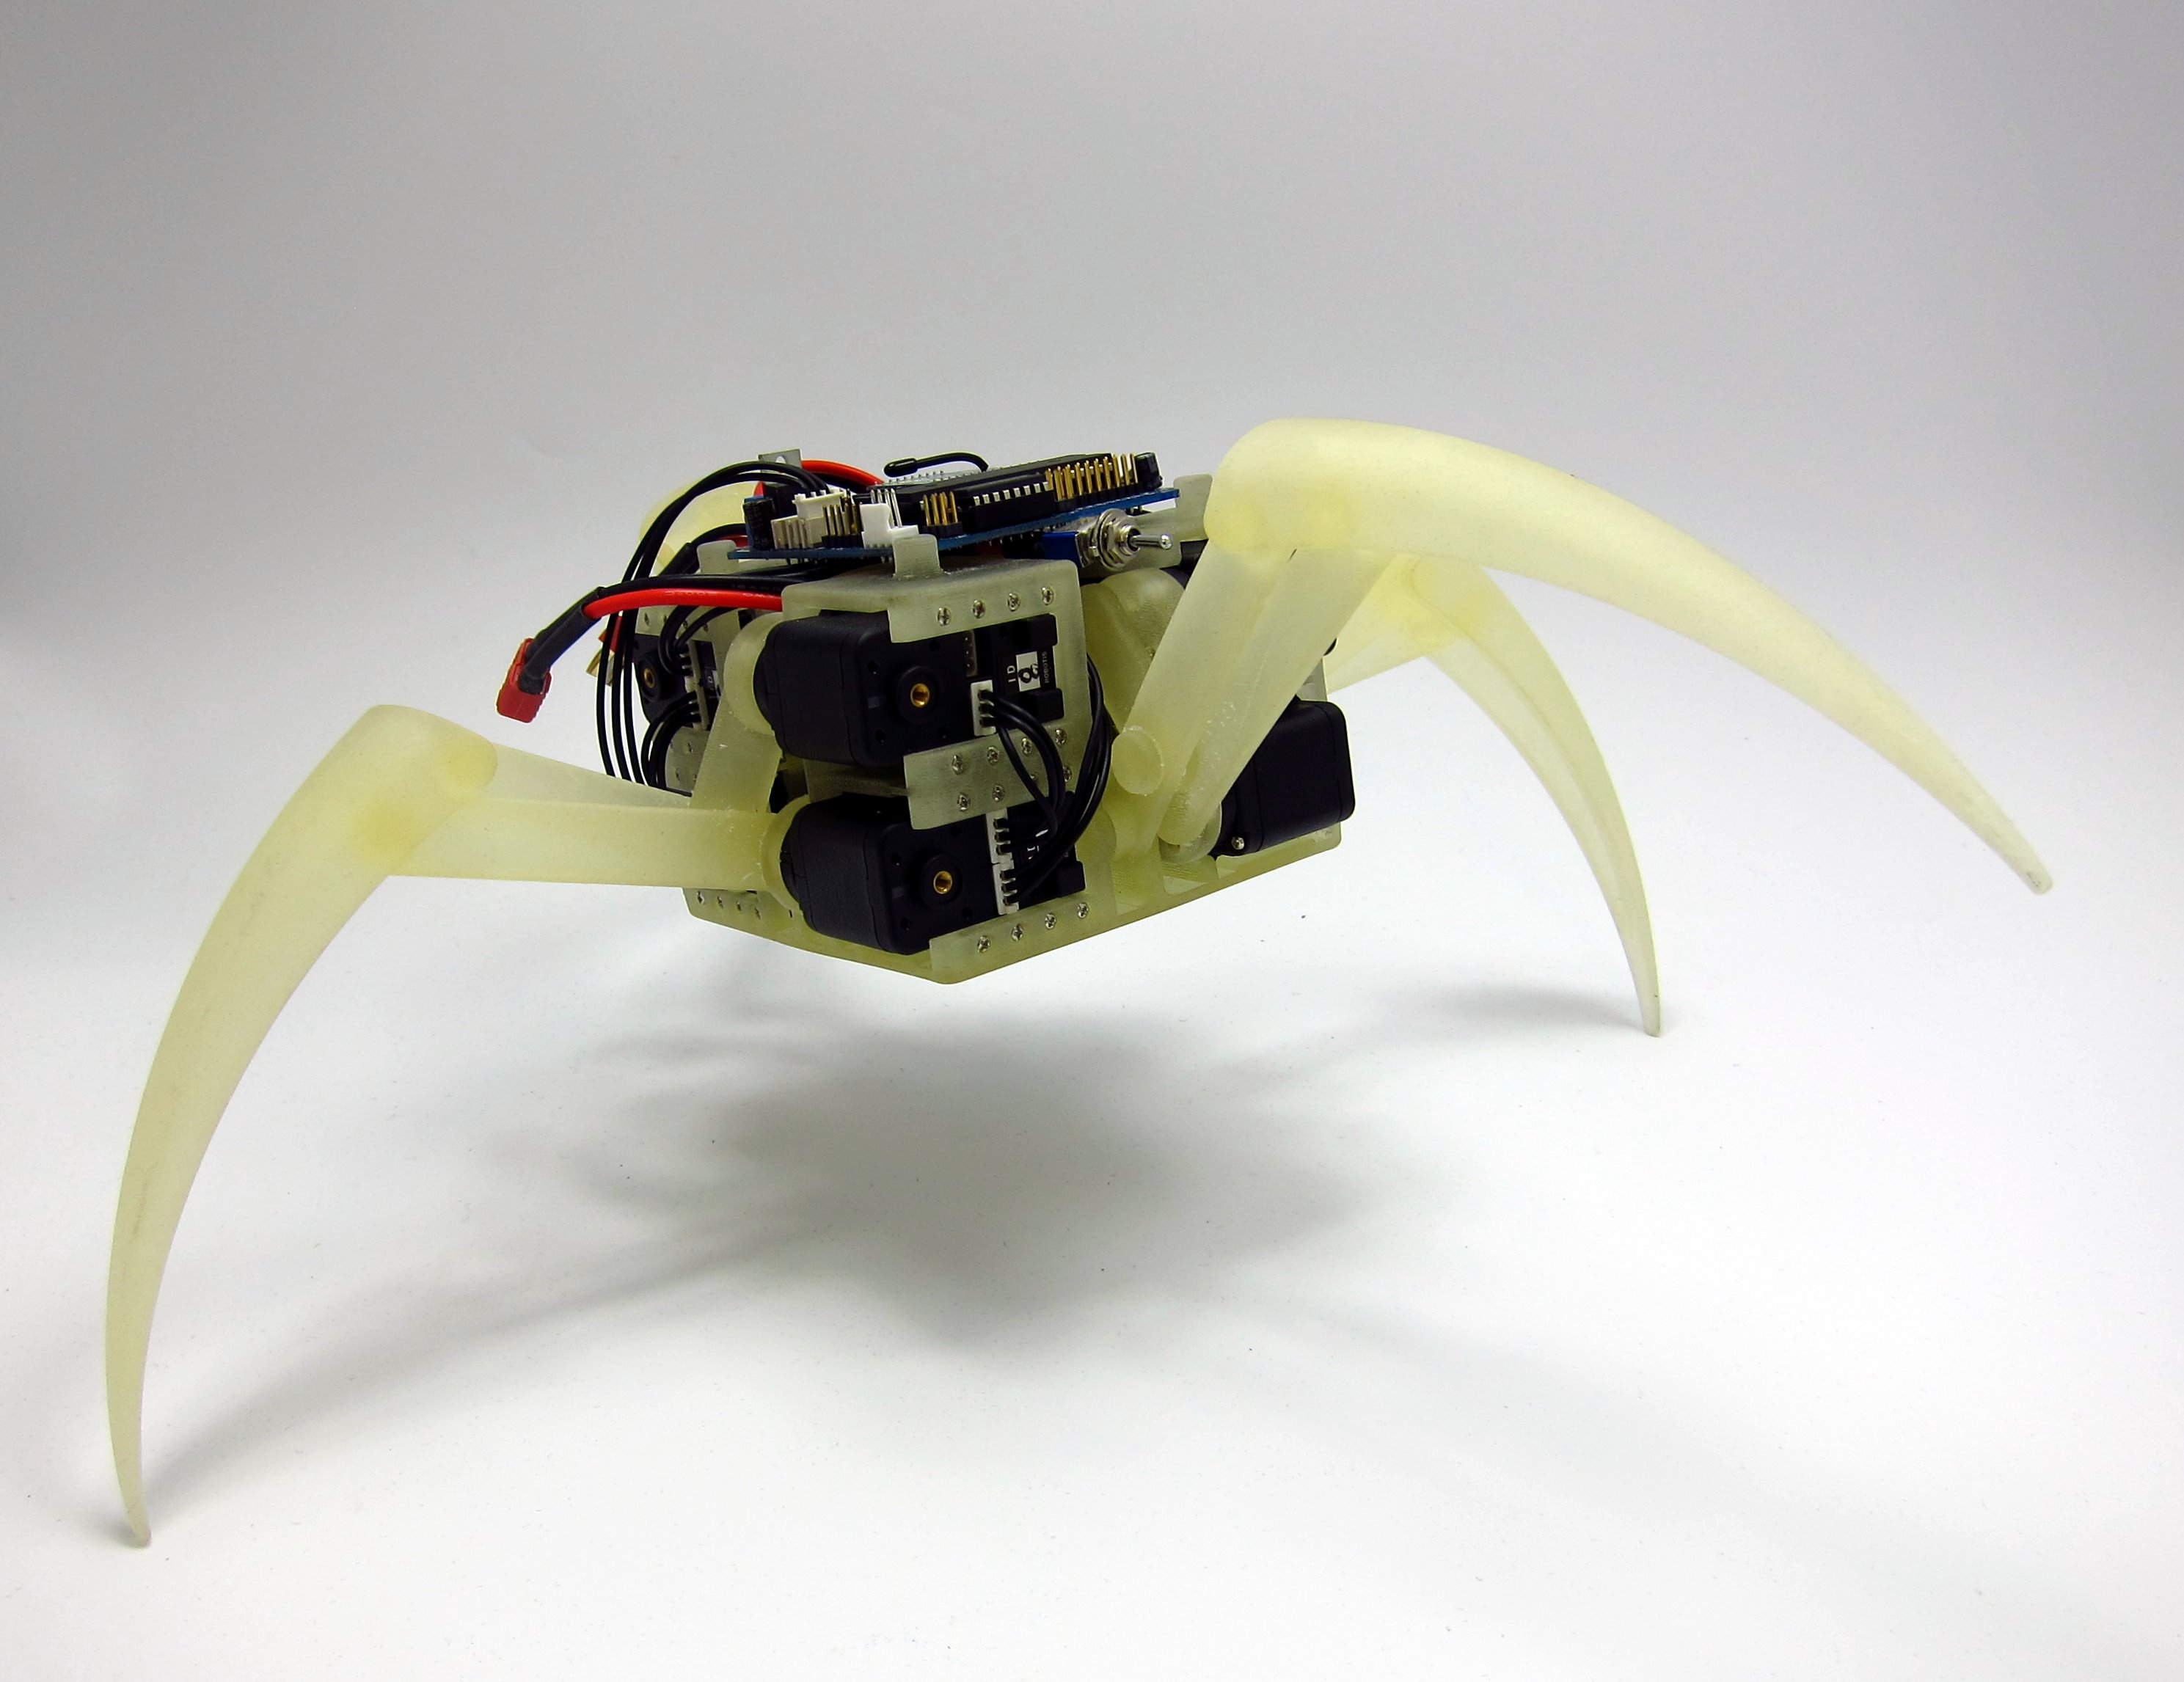
\includegraphics[width=.45\textwidth]{fig1.jpg}
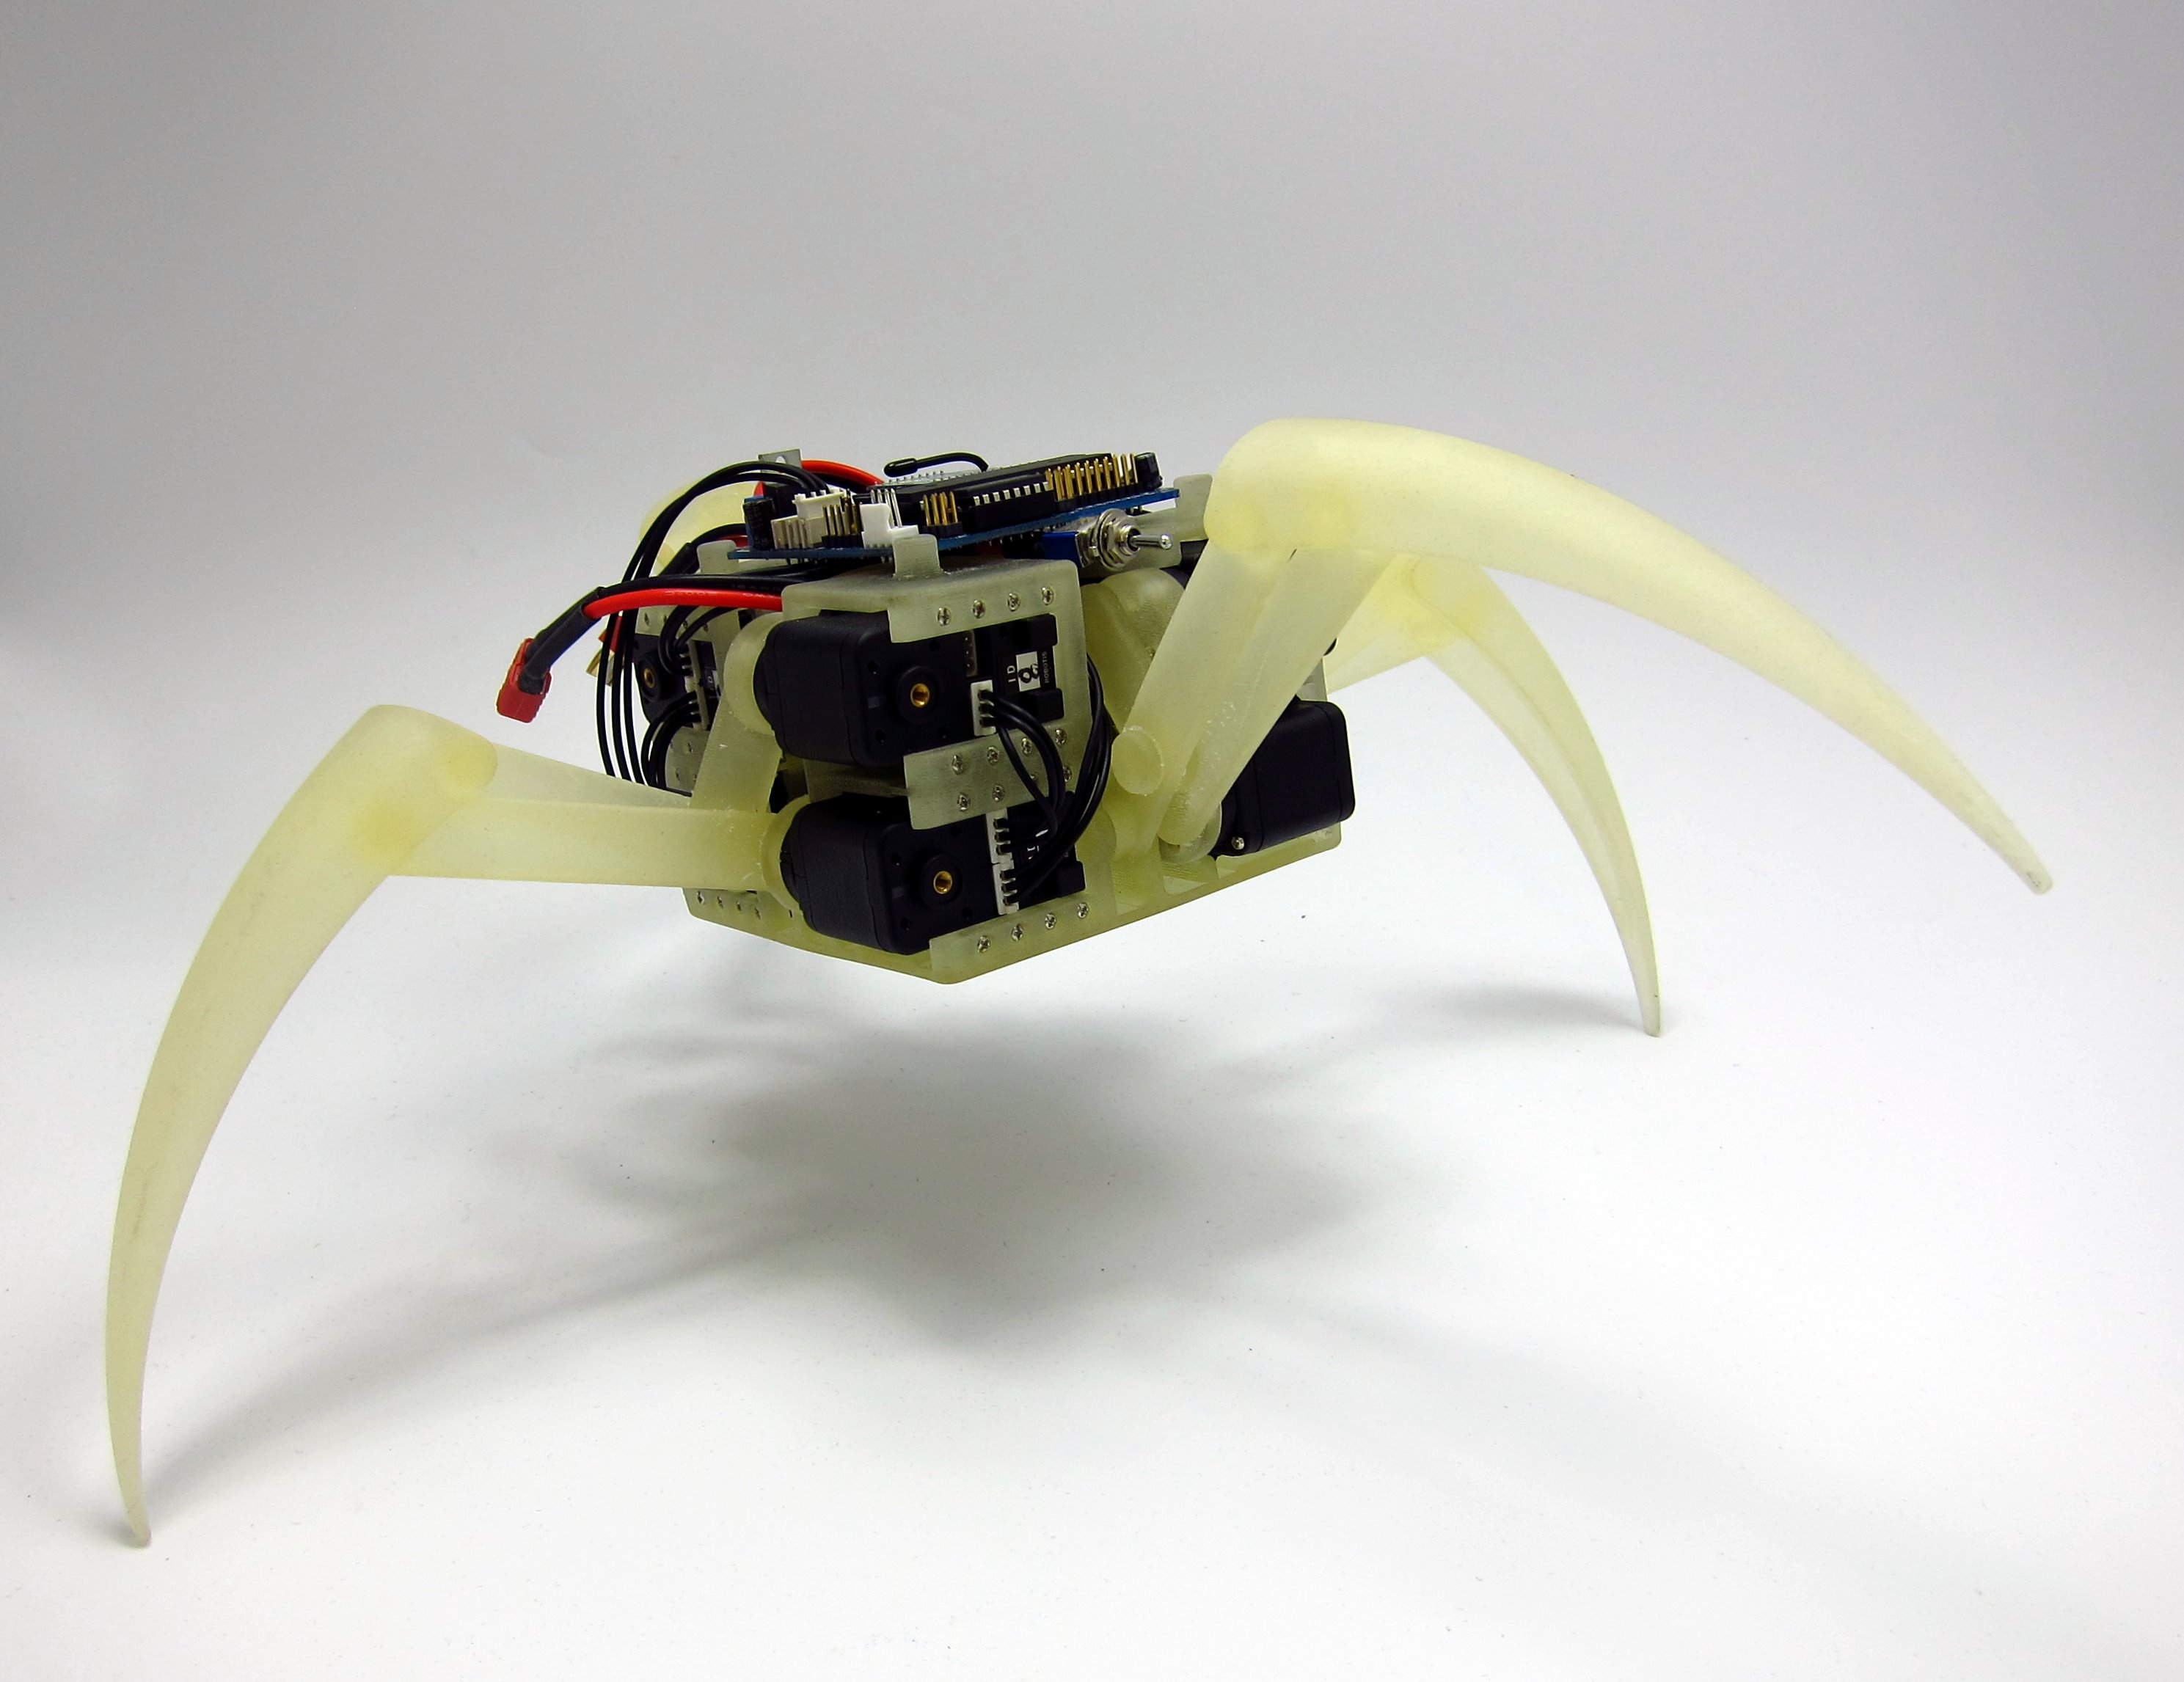
\includegraphics[width=\columnwidth]{fig1.jpg}
\caption{Aracna: an open-sourced quadruped robot platform. All
  instructions and downloads are publicly available at
  http://creativemachines.cornell.edu/aracna .}
\label{fig1}
\end{center}
\end{figure}

The results just mentioned suggest that evolutionary algorithms are a promising approach for generating gaits and other behaviors for physical robots. Despite this promise, the field remains small, partly because robots are expensive and they are difficult to modify. Access to cheap, customizable robots could increase the number of researchers able to participate in the field. Moreover, in nearly all of the papers mentioned previously, the robots were custom-made, preventing teams at other universities from reproducing the results of other groups and or testing new algorithms on a robotic platform used in a previous study. That, in turn, slows the progress of science because it is difficult to interpret whether the variance in results between different studies was due to the algorithms used or the robotic platform those algorithms were tested on.  

Some robot platforms are emerging, but they tend to be wheeled robots without complex kinematics, such as the ePuck~\citep{mondada2009puck}. Wheeled robots are interesting testbeds for many robotic behaviors, but they do not allow gait evolution and are unable to traverse rugged terrains. Legged robotic platforms exist, but they tend to be extremely expensive, such as the Aldebaran Nao, which costs more than \$10,000 USD. Another drawback to these commercial platforms is that it is hard, if not impossible, to modify the hardware design because they are not open-source hardware projects, and complex manufacturing tools would be required to manufacture new parts. 



In this paper we address these needs by introducing \emph{Aracna}, a low-cost, easily customizable robot platform with non-intuitive walking
kinematics~(Figure 1). Aracna is the third quadruped robot developed for evolutionary learning algorithms by the Creative Machines Lab at Cornell University~\citep{HL, JY}. 


A common feature among the quadruped
robots is two actuators that drive the flexion/extension of a knee and
hip joint around parallel axes in each leg. The original Creative
Machines Lab quadruped robot favored starfish-like movements
\citep{HL}. The second quadruped robot --- QuadraTot ---
developed spider-like movements but was found to be limited by its
weight \citep{JY}. When creating the Aracna, we designed the hardware to
complement fast spider-like movements.




\section{Hardware}

\begin{figure}[t]
\begin{center}
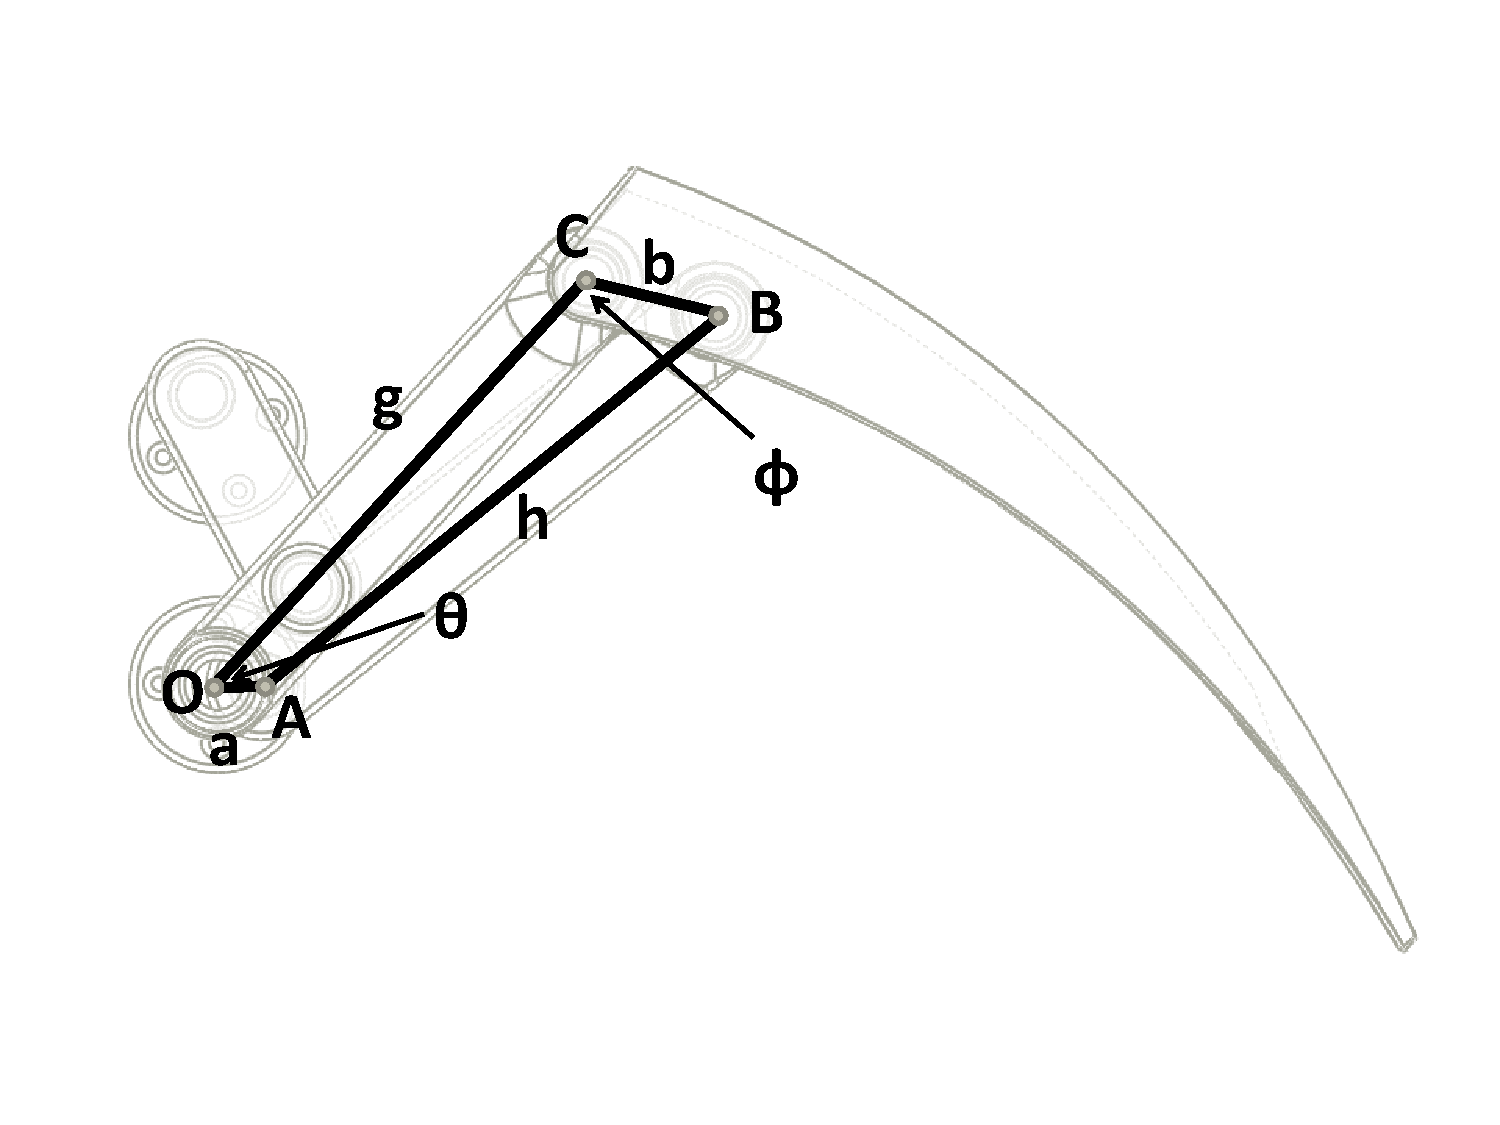
\includegraphics[width=.23\textwidth]{fig3.pdf}
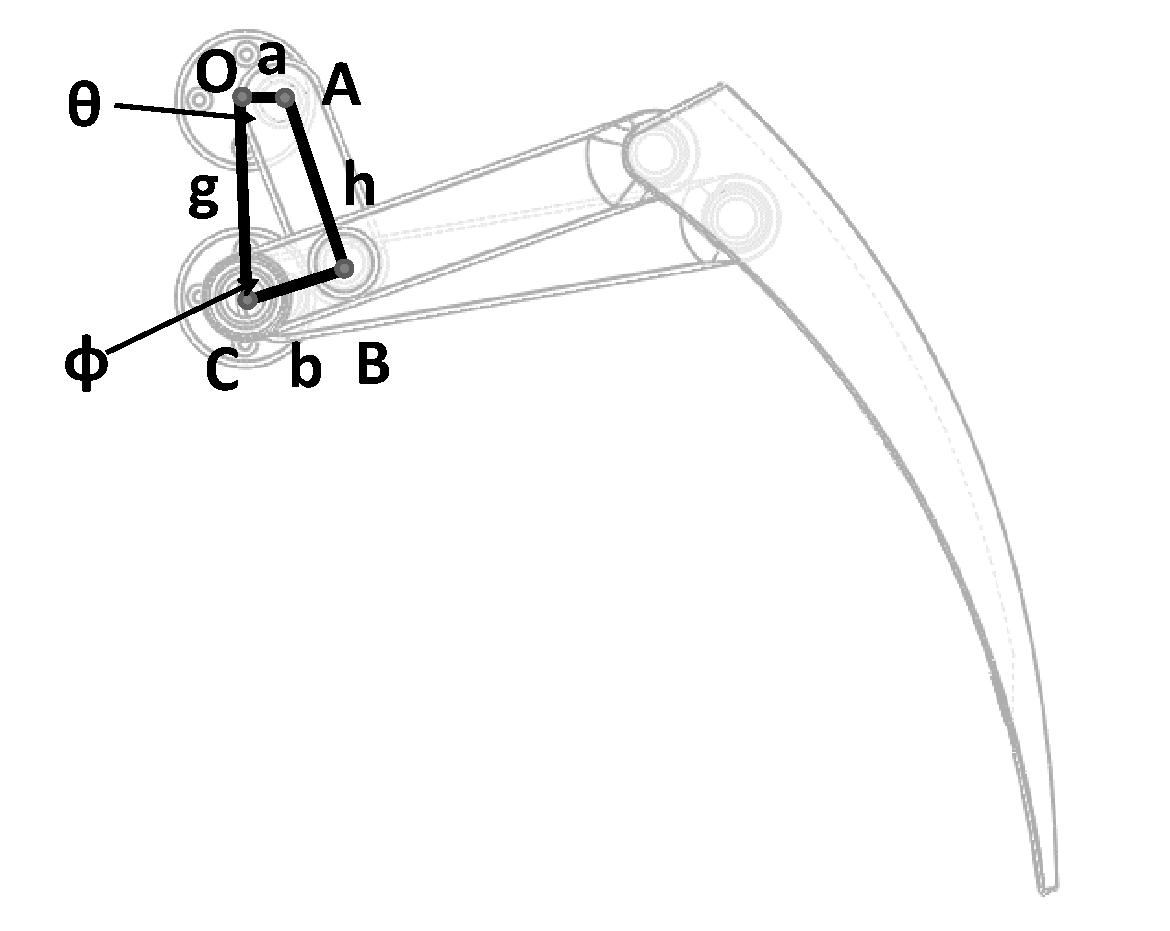
\includegraphics[width=.23\textwidth]{fig4.pdf}
\caption{Crank-rocker four-bar linkage controlling flexion/extension of
  the knee and hip joints. In both cases above, the input crank (link
  OA) is actuated by a servo, the rocker is the leg (link CB), and the
  fixed link is OC.}
\label{fig3}
\end{center}
\end{figure}

%\begin{figure}[t]
%\begin{center}
%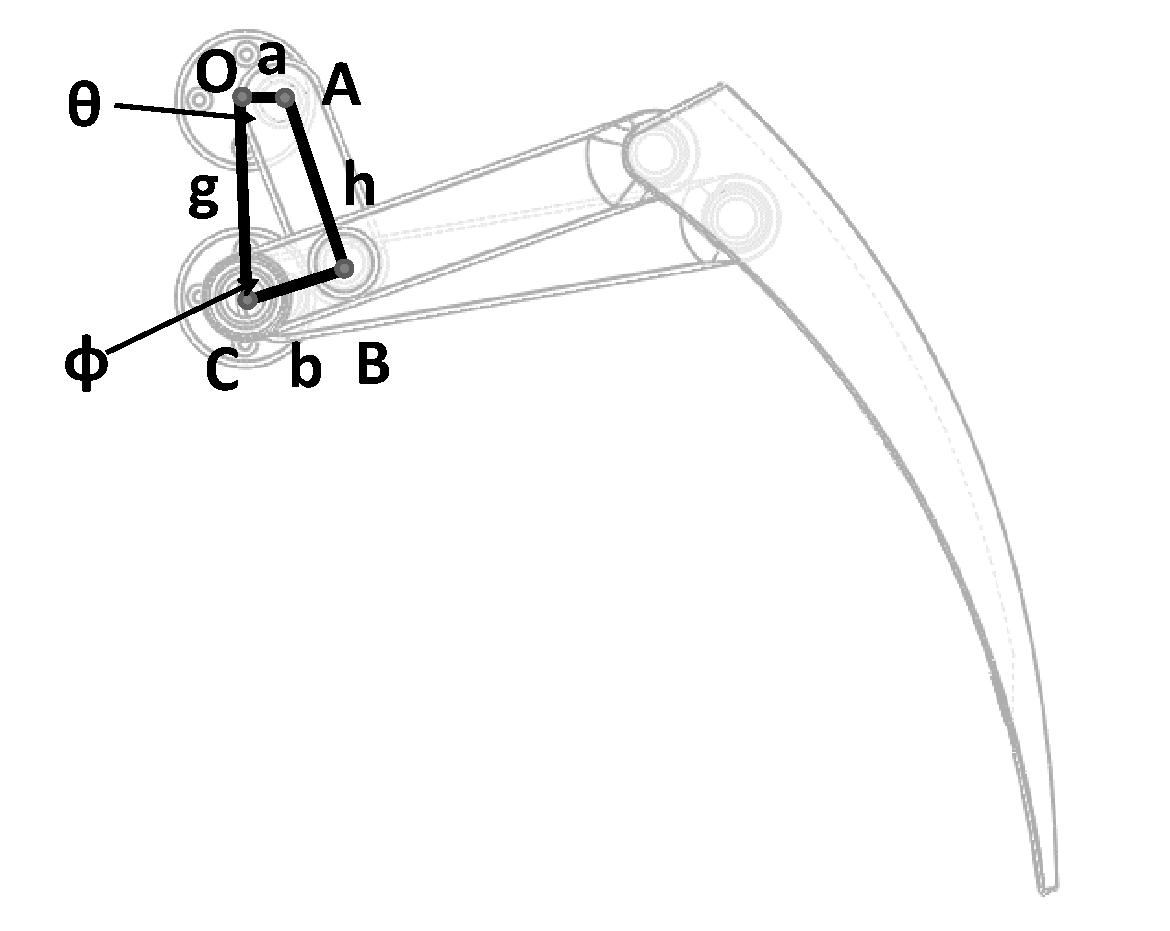
\includegraphics[width=2.25in,angle=0]{fig4.pdf}
%\caption{Crank-rocker four-bar linkage controlling flexion/extension of the hip joint.}
%\label{fig4}
%\end{center}
%\end{figure}

The hardware of Aracna evolved from the previous Creative Machines Lab
quadruped robots. We kept the same two degree of freedom pitch joint
scheme but decreased the weight and constrained the movement of the
joints toward the goal of creating faster spider-like movement. To
prevent starfish-like movement, the legs were constrained. We designed
the robot with two four-bar mechanisms to drive the joints in each
leg. With a four-bar mechanism in place, the leg moves at a fraction
of the output angle of the actuator, giving the motor a relatively
larger mechanical advantage over the position of each leg.
Figure~\ref{fig3} shows the crank-rocker system, where the input crank
is actuated by a servo and the rocker is the leg. In this
configuration, we keep the servo motors contained in the center of the
robot, reducing both the inertia and mass of each leg. The four-bar
mechanisms satisfied the design goal of making a robot that had
non-traditional movements.  To make the robot
accessible as an open-source platform, it was designed to be 3D
printed. The 3D print files and CAD files can be accessed by the
public to be printed and, if desired, modified.

The robot is designed to be lightweight, because previous similar
robots may have been too heavy and underpowered to generate
interesting gaits. We use a single LiPo 11.1V battery to
power 8 Dynamixel AX-18 servo motors and an ArbotiX
microcontroller. The main processing occurs on an external computer,
which allows the robot to have cheaper and lighter components
on-board. The space in the center of the body houses the
battery to reduce material weight and cost. Aracna weighs 1.03 kg.
% 1034g

\begin{figure}[t]
\begin{center}
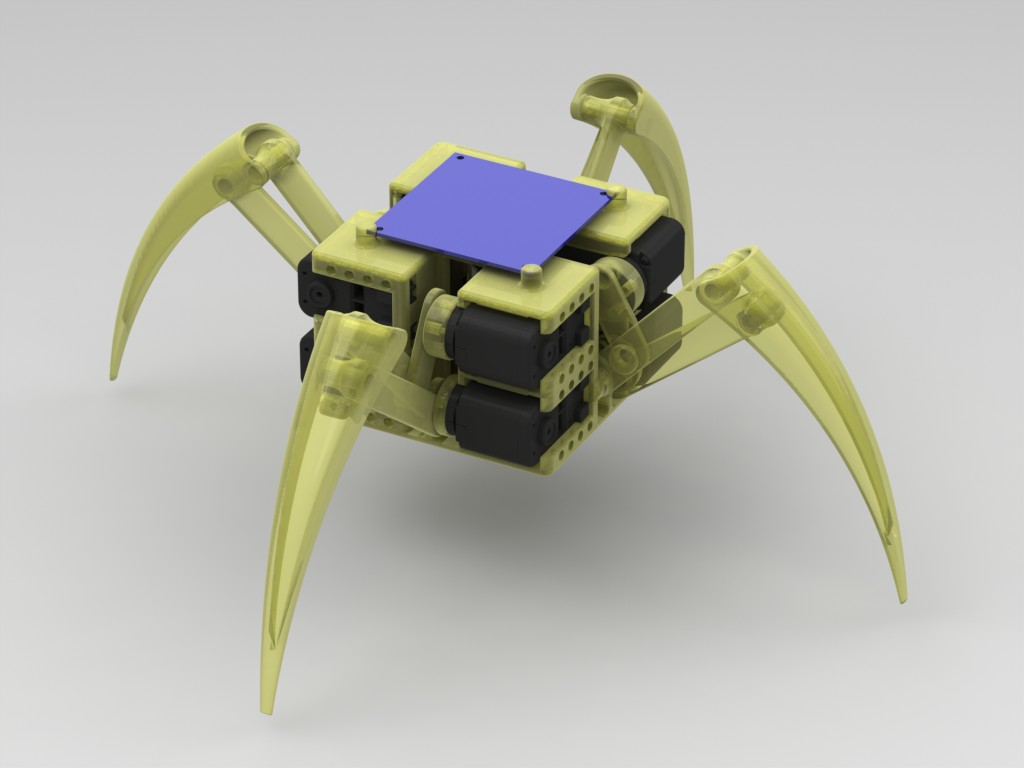
\includegraphics[width=\columnwidth]{fig5.jpg}
\caption{Rendered CAD model of Aracna.}
\label{fi52}
\end{center}
\end{figure}



\section{Software}

The software is open-sourced Python based on the
code developed for the QuadraTot platform \citep{JY}. All code is
available on the project website \citep{WEB}. We use an infrared light
emitting diode (LED) on the robot along with an external Nintendo Wii
remote to provide feedback of the distance traveled. The robot
receives feedback from the Wii remote and internal servo sensors and
then processes the information to send the next command to
the servos. The communication between the external control computer
and the ArbotiX on-board microcontroller occurs over wireless XBee.



\section{Specifications}

\begin{figure}[t]
\begin{center}
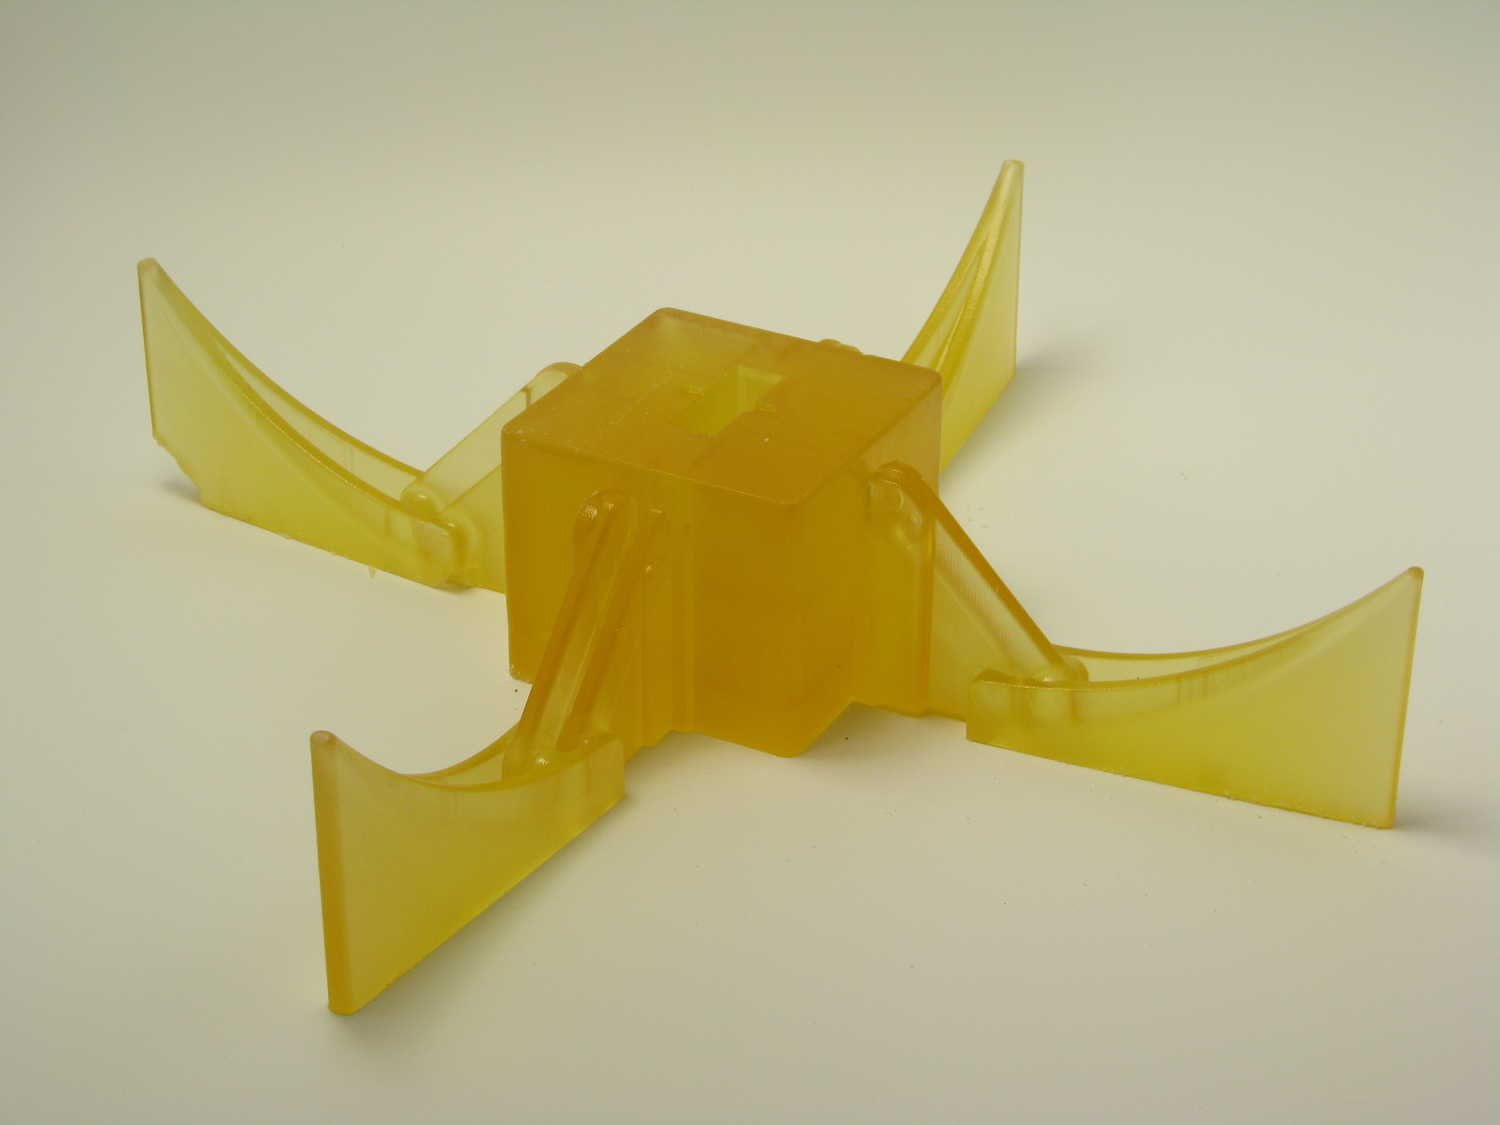
\includegraphics[width=.37\textwidth]{fig2.jpg}
\caption{Robot printed as one piece with support material intact.}
\label{fig2}
\end{center}
\end{figure}

The Aracna may be 3D printed as a single part (Figure~\ref{fig2}). On
an Object Connex500 printer, the robot was completed in 26 hours,
using approximately 1000 g of model material and 1500 g of support
material. We estimated the cost of the printed parts to be \$410 by
using an estimated model material cost of \$1/4.5g and support
material cost of \$1/8g. This cost estimate is variable depending on
the type of material used. The robot has no removable printed parts
except for the battery cover. In the near future, we will make STL files
available for printing the robot as separate parts on
3D printers with smaller tray sizes. Printing the robot as separate parts
will also reduce the amount of support material needed, and thus the
overall cost. As shown in Table~\ref{tab:cost}, the total cost of the
Aracna is just under \$1500; these estimates are based on the material
calculations above and prices from trossenrobotics.com in March 2012.

\begin{table}[h]
\center{
\begin{tabular}{|c|c|}
\hline
Part & Cost\\
\hline\hline
3D Print Materials & \$410\\
ArbotiX Robocontroller Kit & \$189\\
Dynamixel AX-18A Robot Actuator (x8) & \$721\\
3S 11.1V 2000mAh Pro Lite LiPo Battery & \$73\\
LiPo Battery Balance Charger Kit & \$70\\
Cables, Connectors, Misc & \$28\\
\hline\hline
\bf Total & \bf \$1491\\
 \hline
\end{tabular}
}
\vskip 0.25cm
\caption{Estimated total cost. A complete parts list is on our website \citep{WEB}.}
\label{tab:cost}
\end{table}



\section{Acknowledgements}

This work was supported by the National Science Foundation's Office of
Emerging Frontiers in Research and Innovation (grant number 0735953).


\footnotesize
\bibliographystyle{apalike}
\bibliography{references}
\end{document}

